\documentclass[a4paper]{article} 
\addtolength{\hoffset}{-2.25cm}
\addtolength{\textwidth}{4.5cm}
\addtolength{\voffset}{-3.25cm}
\addtolength{\textheight}{5cm}
\setlength{\parskip}{0pt}
\setlength{\parindent}{0in}

%----------------------------------------------------------------------------------------
%	PACKAGES AND OTHER DOCUMENT CONFIGURATIONS
%----------------------------------------------------------------------------------------

\usepackage{blindtext} % Package to generate dummy text
\usepackage{charter} % Use the Charter font
\usepackage[utf8]{inputenc} % Use UTF-8 encoding
\usepackage{microtype} % Slightly tweak font spacing for aesthetics
\usepackage[english, ngerman]{babel} % Language hyphenation and typographical rules
\usepackage{amsthm, amsmath, amssymb} % Mathematical typesetting
\usepackage{float} % Improved interface for floating objects
\usepackage[final, colorlinks = true, 
            linkcolor = black, 
            citecolor = black]{hyperref} % For hyperlinks in the PDF
\usepackage{graphicx, multicol} % Enhanced support for graphics
\usepackage{xcolor} % Driver-independent color extensions
\usepackage{marvosym, wasysym} % More symbols
\usepackage{rotating} % Rotation tools
\usepackage{censor} % Facilities for controlling restricted text
\usepackage{listings, style/lstlisting} % Environment for non-formatted code, !uses style file!
\usepackage{pseudocode} % Environment for specifying algorithms in a natural way
\usepackage{style/avm} % Environment for f-structures, !uses style file!
\usepackage{booktabs} % Enhances quality of tables
\usepackage{tikz-qtree} % Easy tree drawing tool
\tikzset{every tree node/.style={align=center,anchor=north},
         level distance=2cm} % Configuration for q-trees
\usepackage{style/btree} % Configuration for b-trees and b+-trees, !uses style file!
\usepackage[backend=biber,style=numeric,
            sorting=nyt]{biblatex} % Complete reimplementation of bibliographic facilities
\addbibresource{ecl.bib}
\usepackage{csquotes} % Context sensitive quotation facilities
\usepackage[yyyymmdd]{datetime} % Uses YEAR-MONTH-DAY format for dates
\renewcommand{\dateseparator}{-} % Sets dateseparator to '-'
\usepackage{fancyhdr} % Headers and footers
\pagestyle{fancy} % All pages have headers and footers
\fancyhead{}\renewcommand{\headrulewidth}{0pt} % Blank out the default header
\fancyfoot[L]{} % Custom footer text
\fancyfoot[C]{} % Custom footer text
\fancyfoot[R]{\thepage} % Custom footer text
\newcommand{\note}[1]{\marginpar{\scriptsize \textcolor{red}{#1}}} % Enables comments in red on margin

%----------------------------------------------------------------------------------------

\begin{document}

%-------------------------------
%	TITLE SECTION
%-------------------------------

\fancyhead[C]{}
\hrule \medskip % Upper rule
\begin{minipage}{0.295\textwidth} 
\raggedright
\footnotesize
Jaime Andres Torres Bermejo \hfill\\   
202014866\hfill\\
andrestbermejoj@gmail.com
\end{minipage}
\begin{minipage}{0.4\textwidth} 
\centering 
\large 
Proyecto 3\\ 
\normalsize 
Diseño y Análisis de Algoritmos\\ 
\end{minipage}
\begin{minipage}{0.295\textwidth} 
\raggedleft
\today\hfill\\
\end{minipage}
\medskip\hrule 
\bigskip

%-------------------------------
%	CONTENIDO
%-------------------------------
\section{Enunciado del Proyecto}
\textbf{Democracia representativa en Pandora}

En un pais llamado Pandora se tiene una democracia representativa en la que se forma un
congreso con políticos que representan a los ciudadanos. Gracias a análisis de información de
redes sociales, se puede predecir con qué políticos se sentiría representado cada ciudadano. Dado
que cada congresista recibe un sueldo, usted ha sido contratado para determinar cual es el número
mínimo de congresistas que deben hacer parte del congreso para que todos los ciudadanos se
sientan representados.

\paragraph{Problema:}
Dados N ciudadanos, M políticos, y por cada ciudadano una lista de los políticos con los que el
ciudadano se sentiría representado, determinar cual es la mínima cantidad de políticos necesarios
para representar a todos los ciudadanos de Pandora y quienes podrían ser dichos políticos.

\paragraph{Ejemplo:}
Dado N=8, M=5 y la siguiente lista de políticos por cada ciudadano:

Ciudadano 1: {1, 3, 5}

Ciudadano 2: {2, 5}

Ciudadano 3: {1, 2, 4}

Ciudadano 4: {2, 3, 4}

Ciudadano 5: {1, 5}

Ciudadano 6: {1, 4, 5}

Ciudadano 7: {3, 4}

Ciudadano 8: {3, 5}

La respuesta sería de longitud 2 porque por ejemplo los políticos 4 y 5 representarían a todos los ciudadanos

OUTPUT: [4,5]
%------------------------------------------------
\section{Especificaciones del proyecto}

\subsection{Entorno de Desarrollo y entorno de prueba.}

Dada la necesidad de un desarrollo relativamente rápido, elegí Python para este proyecto, dado que es un 


\begin{itemize}
    \item \textbf{Sistema Operativo: } Ubuntu/Kubuntu 22.10 x86\_64, Minimal Install. También probado con Fedora
    Linux 38 Workstation x86\_64, por lo tanto se sabe que el programa en teoría podría correr en distribuciones basadas en Debian,
    Red Hat Linux o Arch Linux, no tengo un computador con Mac OS X o BSD para probar con otros sistemas Unix
    \item \textbf{Kernel: }Linux 5.19.0-38-generic y 6.2.0
    \item \textbf{Lenguaje de Programación: }Python 3.11.7 x86\_64, Compilado desde apt, incluye python3-pip,
    También probado con la versión de Arch y DNF (el manejador de paquetes de Fedora/RHEL)
    \item \textbf{Librerías Utilizadas}
    \begin{itemize}
        \item os
        \item itertools
    \end{itemize}
    \item \textbf{Procesador: }AMD Ryzen 5 3550H with Radeon Vega Mobile Gfx (8) @ 2.100GHz 
    \item \textbf{IDE: } Visual Studio Code 1.76.2, instalado desde un paquete snapd. Incluye extensiones
    de Git y Python. En Manjaro fue instalado desde el AUR con el paquete visual-studio-code-bin
\end{itemize}

\subsection{Estructura del Input y Output}
A primera vista, este pareciese ser un problema bastante extraño, el input no pareciese seguir una estructura tan
concreta como aquella de los primeros 2 proyectos, sin embargo, al extraer los valores 'N' y 'M' al inicio de cada
caso, es mucho mas sencillo de leer. El ejemplo de este input proveido es:

\begin{verbatim}
    3
    8 5
    1 3 5
    2 5
    1 2 4
    2 3 4
    1 5
    1 4 5
    3 4
    3 5
    5 5
    1 2
    4 5
    3 4
    2
    3 5
    3 3
    1 2
    2
    2 3
\end{verbatim}

como puede verse, no hay una estructura concreta para cada array. Esto se debe a que estos son 
arrays cuya longitud esta no predeterminada, sino establecida por la cantidad de políticos
que representan a un ciudadano concreto: En otras palabras, esto esta representando no uno, sino 
dos grafos diferentes. Esto es un poco abstracto al inicio, pero tiene sentido al separarse en 
ciudadanos y políticos. Estos dos grafos estan interconectados por una lista de adyacencia, donde
se guardan las preferencias de los ciudadanos hacia los politicos y los representados por cada politico.
Estos dos grafos se interconectan uno con nodos del otro, y se referencian constantemente en la solución
propuesta.

\subsection{Lectura de datos}
Según se nos fue informado por los monitores, la lectura se hará a partir de la lectura
de archivos de texto y, por lo tanto, la estructura del archivo de Python esta pensada para
poder leer varios archivos de texto secuencialmente. Para esto hemos importado la librería 'os'
de las librerías base de Python. la estructura es bastante similar a aquella del primer proyecto.
Sin embargo, la división de casos se hace de forma diferente, dado que a diferencia de dicho Proyecto,
toma varios arrays dentro de un solo caso. Cada caso es conformado por una cantidad 'N' de Arrays.
A partir de esta se puede 
%------------------------------------------------
\section{Diseño de la Solución}
\subsection{Conceptos Teóricos Importantes}
\subsubsection{NP Completitud}

Un problema es NP-Completo si:
\begin{itemize}
    \item es un problema de decision.
    \item se puede demostrar en tiempo polinomial cuando la respuesta es si.
    \item un algoritmo de fuerza bruta puede encontrar todas las soluciones.
    \item pcional: desciende o puede demostrarse a partir de la prueba formal de otro algoritmo
  
    Esta solucion cumple con todas estas opciones si se toma la decision de "este set de candidatos representa
    todos los ciudadanos" como un problema de decisión y desciende de Vertex Cover, que es NP-C, por lo que se 
    califica dentro de la categoría.
\end{itemize}

\subsection{Conceptos Prácticos Importantes}
\subsubsection{Tipado dinámico}
El lenguaje de Programación utilizado para resolver este algoritmo fue Python,
el cuál tiene la capacidad de mantener una estructura de tipado dinámica, esta
implica que podemos declarar una variable de un tipo y esta podrá ser interpretada
como de otro tipo a la hora de compilar el código, otros lenguajes de Programación
con esta carácteristica son Ruby y Javascript. Esto es importante para este problema
porque estamos constantemente convirtiendo los tipos de los valores dados.

\subsection{Problemas similares}
\subsubsection{Vertex Cover}
Este problema desciende de Vertex cover, definido cómo [2]:
\begin{center}
    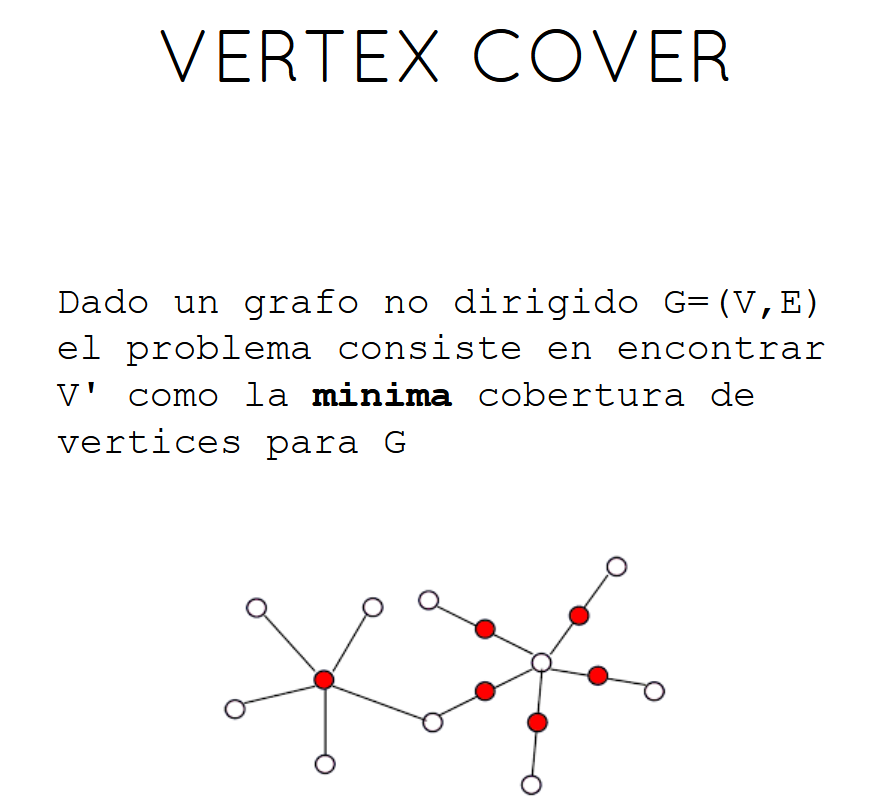
\includegraphics[scale=0.5]{vcover.PNG}    
\end{center}
donde se busca la cobertura mínima de vertices para acceder a todo el grafo. En 
este problema, sin embargo, se usa un grafo diferente para lograr acceder a la cobertura
del grafo a evaluar, en lugar de usar los nodos de un solo grafo para resolver el problema.

\paragraph{Estrategia de solución}
Este problema por si mismo puede aproximarse de forma la cuál nos dé una solución
de máximo el doble del tamaño de la solución óptima con el siguiente algoritmo:
\begin{center}
    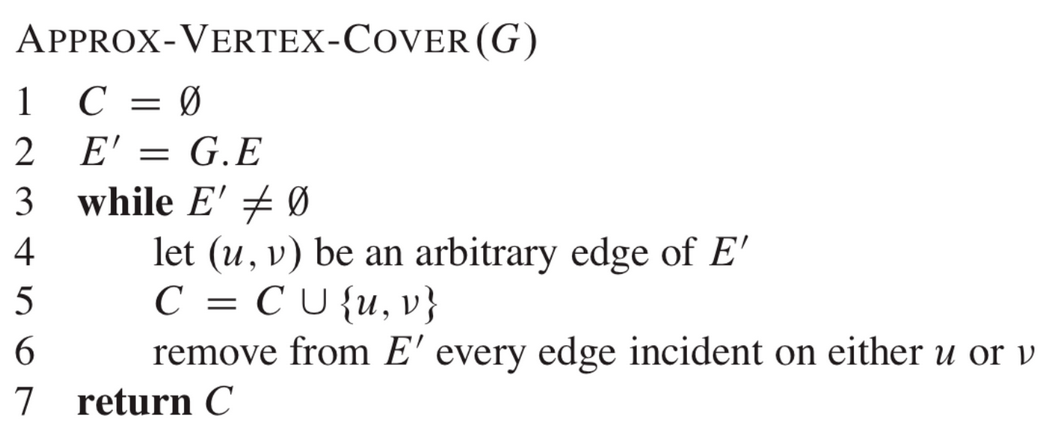
\includegraphics[scale=0.5]{aprox.PNG}    
\end{center}

Dada la exactitud del resultado esperado, sin embargo, no se va a poder hacer esta
aproximación en este caso, por lo cual aprovechando la NP-Completitud del caso, usaremos
combinaciones y fuerza bruta para lograr solucionar este problema con un resultado óptimo,
donde entre menor la longitud del array a ser respuesta, menor es el tiempo de ejecución.


\subsection{La Solución}
\subsubsection{Mantras de diseño}
\begin{itemize}
    \item \textbf{El problema es NP-Completo: }
    Como ya fue explicado, este problema es una versión alternativa de vertex cover. Por lo que el 
    problema va a ser NP-C, y la solución funcionará polinomialmente.
    \item \textbf{Es una solución especifica: } lastimosamente, no podemos utilizar una solución aproximada aunque
    Vertex Cover sea un algoritmo aproximado dada la especificación de que este algoritmo tiene que
    encontrar la solución óptima. 
    \item \textbf{Hay dos grafos: } Para la solución propuesta, se convierte el input a dos grafos 
    separados. dentro de un grafo, las conexiones no apuntan a otros nodos dentro del mismo sino a 
\end{itemize}

\subsubsection{Código Fuente}
\begin{verbatim}
    #Problema detectado: vertex cover
    def solve(n, m, caso):

        politician_graph = {}
        citizen_graph = {}
        #generación primer grafo
        for i in range(n):
            citizen_graph[i+1] = caso[i]
        
        #generación segundo grafo.
        for i in range(1, m+1):
            citizens_into = []
            for j in range(1, n+1):
                check = citizen_graph[j]
                if i in check:
                    citizens_into.append(j)
            politician_graph[i] = citizens_into

        i = 1
        while i < m:
            comb = combinations(politician_graph.keys(), i)
            for j in comb:
                voteset = []
                for k in j:
                    voteset.extend(politician_graph[k])
                if len(set(voteset)) == n:
                    return j
            i += 1
\end{verbatim}

%------------------------------------------------
\section{Análisis de la Solución}

\subsection{Complejidad}
Nota: es posible que operaciones de entrada/salida y lectura/escritura fuera de la función 
principal en esta solución aumenten su tiempo de ejecución.

Temporal: Dado el uso de combinaciones para lograr esta solución, la complejidad temporal es $ O( r * [nCr]) $
Espacial: $ O(n^2) $, por la creación de los grafos.
\subsection{Casos Hipotéticos.}
\paragraph{Suponga que conociendo el partido político al que pertenece cada político se
quiere asegurar que haya al menos k partidos representados.}

A la hora de hacer las combinaciones, podemos filtrar el resultado a aquellos cuyo 'set' de
partidos que se podría sacar por medio de la función 'filter' de python, cuyos especificos dependerían
de la estructura del input y que sería de complejidad O(n). Se reemplaza el sistema de combinaciones filtrado
y se opera con normalidad.

\paragraph{Suponga que se determina que cada ciudadano se siente representado por
máximo dos políticos.}

Esta restricción técnicamente nos permitiría resolver el problema exactamente igual que como se resuelve acá, sin
embargo, hay algunas optimizaciones que se abren a partir de esta restricción dado que con esta restriccion podemos
intentar triangular el número de políticos que serán parte del sistema de soluciones anteriormente a computar las
combinaciones. Esto reduciría significativamente el tiempo de ejecución de la aplicación pero no necesariamente
su complejidad.


\subsection{Limitantes}
    \begin{itemize}
        \item el archivo solo puede recibir inputs de archivos de texto, un input no
        puede ser ingresado directamente desde el usuario a partir de la consola
        \item la necesidad de un Output exacto limita las capacidades de optimización de 
        este algoritmo.
    \end{itemize}
\subsection{Consideraciones}
\begin{itemize}
    \item La capacidad de tipado dinámico de Python es directamente responsable de
    la capacidad de este algoritmo en algunos casos, gran parte de las funciones deberían reescribirse en caso de que se fuese a reescribir la solución
    en un sistema de tipado estático.
    \item Este programa asume un input correcto
    \item por ultima vez, este es un trabajo en grupo que realicé solo, por favor ten eso
    en cuenta, profe.

\end{itemize}
%------------------------------------------------
\section{Referencias.}
\begin{itemize}
    \item [1]: \textit{Enunciado del proyecto, ISIS 1105 Diseño y Análisis de Algoritmos
    Semestre 2023-10. Proyecto – PARTE 3} Uniandes, 2023.
    \item [2] \textit{diaspositivas de clase.}
\end{itemize}
\end{document}
